\documentclass[12pt, titlepage]{article}

\usepackage{booktabs}
\usepackage{tabularx}
\usepackage{hyperref}
\usepackage{graphicx}
\usepackage{float}



\hypersetup{
    colorlinks,
    citecolor=black,
    filecolor=black,
    linkcolor=red,
    urlcolor=blue
}
\usepackage[round]{natbib}

\title{SE 3XA3: Software Requirements Specification\\Title of Project}

\author{Team \#115, AAA Solutions
		\\ Abdallah Taha and tahaa8
		\\ Student 2 name and macid
		\\ Student 3 name and macid
}

\date{\today}

\begin{document}

\maketitle

\pagenumbering{roman}
\tableofcontents
\listoftables
\listoffigures

\begin{table}[bp]
\caption{\bf Revision History}
\begin{tabularx}{\textwidth}{p{3cm}p{2cm}X}
\toprule {\bf Date} & {\bf Version} & {\bf Notes}\\
\midrule
Date 1 & 1.0 & Notes\\
Date 2 & 1.1 & Notes\\
\bottomrule
\end{tabularx}
\end{table}

\newpage

\pagenumbering{arabic}

This document describes the requirements for ....  The template for the Software
Requirements Specification (SRS) is a subset of the Volere
template~\citep{RobertsonAndRobertson2012}.  If you make further modifications
to the template, you should explicity state what modifications were made.

\section{Project Drivers}

\subsection{The Purpose of the Project}

\subsection{The Stakeholders}

\subsubsection{The Client}

\subsubsection{The Customers}

\subsubsection{Other Stakeholders}

\subsection{Mandated Constraints}

\subsection{Naming Conventions and Terminology}

\subsection{Relevant Facts and Assumptions}

User characteristics should go under assumptions.

\section{Functional Requirements}

\subsection{The Scope of the Work and the Product}

\subsubsection{The Context of the Work}
\begin{figure}[H]
\caption{Work Context}
\centering
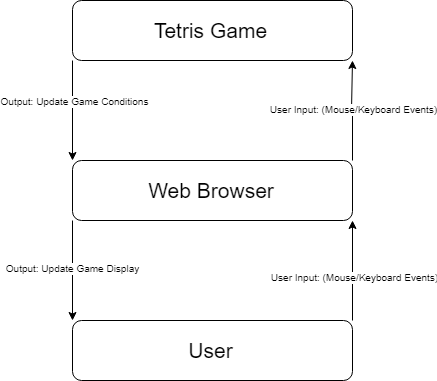
\includegraphics[width=0.95\linewidth]{Context.png}
\end{figure}


\subsubsection*{Work Partitioning}
\begin{table}[H]
\caption{Work Partitioning Part I}
\hskip-2.5cm\begin{tabular}{|c|c|c|c|}
\hline
Event Number & Event Name & Input & Output\\
\hline
1 & Tetris game Creation & Developer code & Web Browser\\
\hline
2 & Tetris game Audio & Microphone & Audio output device\\
\hline
3 & Tetris Full Row of Blocks & Developer graphics and code & Web Browser\\
\hline
4 & Blocks Overflow Outside of Grid & Developer code & Web Browser\\
\hline
5 & Tetris Score Calculation & Developer code & Web Browser\\
\hline
6 & Tetris Game Final Revision & Developer code & Web Browser\\
\hline
\end{tabular}
\label{default}
\end{table}%

\begin{table}[H]
\caption{Work Partitioning Part II}
\hskip-2.5cm\begin{tabular}{|c|c|}

\hline
Event Number & Summary of BUC\\
\hline
1 & Recreate a terminal based game that works on multiple web browsers\\ 
\hline
2 & Record sound effect to be displayed in the game\\
\hline
3 & Create different functions to perform the game mechanics in this project\\
\hline
4 & Create overflow detection when blocks fall outside of grid then display an end screen\\
\hline
5 & Create a detection system for when row is full and calculate current score\\
\hline
6 & Finishing edits to the project\\
\hline

\end{tabular}
\label{default}
\end{table}%


    
    
\subsubsection{Individual Product Use Cases}

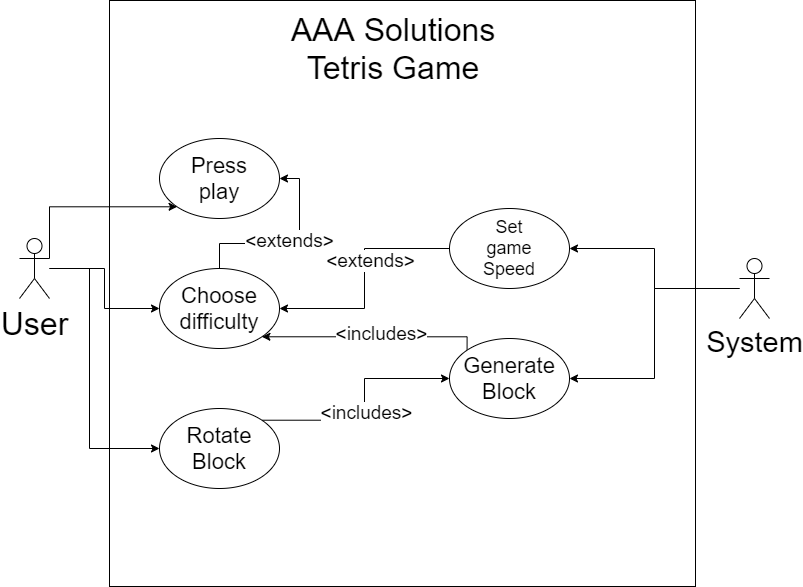
\includegraphics[width=0.95\linewidth]{usecasexa3.png}

\subsection{Functional Requirements}
\begin{itemize}
    \item
    Executable HTML file will launch in a new web browser window.    \subitem
    Fit Criterion or Test Case: \\
    Check if a new tab opens within the web browser when aforementioned HTML file is executed.    
    \item
    The HTML will be executable by any browser with JavaScript compatibility.    \subitem
    Fit Criterion or Test Case: \\
    Execute the HTML file with different major browsers and check if it executes properly.    
    \item
    Initial condition of the game will display a start menu and stay in a standby sate until it receives user input.    \subitem
    Fit Criterion or Test Case: \\
    Check that the game stays in the start menu when executed until it receives an input.    
    \item
    When the game starts the game state will have zero blocks within the grid and score will be set to zero.    \subitem
    Fit Criterion or Test Case: \\
    Check the display of the grid and scoreboard when begin game to check is score is at 0 and no blocks are in the grid.    
    \item
    Blocks will start flowing one by one onto the grid and will rotate based upon user input when the user pushed the play game button.    \subitem
    Fit Criterion or Test Case: \\
    Click play on the game and check that the blocks begin flow onto grid one by one and input the WASD keys to check for the 90-degree rotation.    
    \item
    During the game if a block lands outside of the grid of the game then the game will terminate and display final score to the user.    \subitem
    Fit Criterion or Test Case: \\
    Check that the game returns the users final score and displays the game over screen.    
    \end{itemize}
    



\section{Non-functional Requirements}

\subsection{Look and Feel Requirements}
\subsubsection{Appearance Requirements}
\begin{itemize}
\item The user interface shall be well formatted and separated based on score and game grid.
\item The user interface will include the company logo.
\item The user interface will have different colors for different shaped blocks
\item The user interface will have a distinguished game grid section and separate current score section
\end{itemize}
\subsubsection{Style Requirements}
\begin{itemize}
    \item The user interface will have a consistent font throughout
    \item Blocks will generate and fall seamlessly onto the game grid
    \item Button should be easily identified and responsive 
\end{itemize}

\subsection{Usability and Humanity Requirements}
\subsubsection{Ease of Use Requirements}
The game shall be playable by any user with basic understanding of navigating a web browser.
\subsubsection{Personalization and Internationalization Requirements}
N/A
\subsubsection{Learning Requirements}
A user shall be able to fully understand the game withing five minutes of executing the program.
\subsubsection{Understandability and Politeness Requirements }
The system shall use text to indicate that an action can be performed and shall only use icons when the icon is commonly associated with a standard action (i.e trashcan icon for delete)
\subsubsection{Accessibility Requirements}
This game will be playable to any user that can operate a mouse and keyboard and has access to a web browser.
\subsubsection{Convenience Requirements}
Game will automatically display the play again button for the user when the game ends.


\subsection{Performance Requirements}
\subsubsection{Speed and Latency Requirements}
System shall take no longer then 5 seconds to set up the game once the play button has been pressed. System shall also display the game over menu and calculate the final score in under 3 seconds of game ending.
\subsubsection{Safety-Critical Requirements}
N/A
\subsubsection{Precision or Accuracy Requirements}
Score shall have zero decimal points and will always be a whole number.
\subsubsection{Reliability and Availability Requirements}
System shall go down for no longer then 10 hours every 2 years.
\subsubsection{Robustness or Fault-Tolerance Requirements}
N/A
\subsubsection{Capacity Requirements}
System shall only record previous games score and the current highscore.
\subsubsection{Scalability or Extensibility Requirements}
N/A
\subsubsection{Longevity Requirements}
Expected lifetime of the system shall be indefinite.

\subsection{Operational and Environmental Requirements}
\subsubsection{Expected Physical Environment}
This application shall run on any device with a web browser and a internet connection.
\subsubsection{Wider Environment Requirements}
N/A
\subsubsection{Requirements for Interfacing with Adjacent Systems}
N/A
\subsubsection{Productization Requirements}
N/A
\subsubsection{Release Requirements}
Yearly software releases will be deployed to maintain and improve the application based on client demands and needs.

\subsection{Maintainability and Support Requirements}
\subsubsection{Maintenance Requirements}
Maintenance should only take one day requiring the application to only be down one day at a time.
\subsubsection{Supportability Requirements}
Product should ensure that any device running a web browser should have capability to run the game.
\subsubsection{Adaptability Requirements}
N/A

\subsection{Security Requirements}
\subsubsection{Access Requirements}
Any user can have access to the UI of the product given they have a internet connection and a web browser. Only developers will have access to the backend code of the system.
\subsubsection{Integrity Requirements}
No user shall be able to modify game mechanics or alter scoring for the game.
\subsubsection{Privacy Requirements}
Program shall not release any data other then game data to users.
\subsubsection{Audit Requirements}
N/A
\subsubsection{Immunity Requirements}
N/A


\subsection{Cultural Requirements}
\subsubsection{Cultural Requirements}
This product will have zero references pertaining to religions, ethnic groups or any cultures. This application will be hosted in North America put will have access to anywhere in the world providing they have a internet connection and a web browser.

\subsection{Legal Requirements}
\subsubsection{Legal Compliance Requirements}
The game will be in complice with all laws and regulations.
\subsubsection{Standards Compliance Requirements}
This game shall adhere to the MIT Open Licence.

\subsection{Health and Safety Requirements}
This product will ensure that it was compatible with night mode to protect users eyesight. The product will also ensure that all sound effect remain under 70dB to ensure no damage to hearing. 

\section{Project Issues}

\subsection{Open Issues}

\subsection{Off-the-Shelf Solutions}

\subsection{New Problems}

\subsection{Tasks}

\subsection{Migration to the New Product}

\subsection{Risks}

\subsection{Costs}

\subsection{User Documentation and Training}

\subsection{Waiting Room}

\subsection{Ideas for Solutions}

\bibliographystyle{plainnat}

\bibliography{SRS}

\newpage

\section{Appendix}

This section has been added to the Volere template.  This is where you can place
additional information.

\subsection{Symbolic Parameters}

The definition of the requirements will likely call for SYMBOLIC\_CONSTANTS.
Their values are defined in this section for easy maintenance.


\end{document}